% !TeX TS-program = xelatex
\documentclass[10pt,a4paper]{article}

\usepackage[fontset=fandol, UTF8]{ctex}
\usepackage{fontspec}


\usepackage[margin=2cm]{geometry}
\usepackage[utf8]{inputenc}
\usepackage[T1]{fontenc}
\usepackage{listings}
\usepackage{enumitem}
\usepackage{color}
\usepackage{graphicx}
\usepackage{hyperref}
\usepackage{fourier}
\usepackage[scaled = 0.75]{beramono}
\usepackage{fancyhdr}
\usepackage{tikz}
\pagestyle{fancy}
\definecolor{myltgray}{rgb}{0.95,0.95,0.95}
\usepackage{textcomp}
\usepackage{multicol}
\usepackage{comment}
\rhead{\raisebox{0.66ex}{\thepage}}
\lhead{\raisebox{0.66ex}{Julia 学习笔记}\ \ 
\includegraphics[width=0.409cm]{pen.png}}
\cfoot{}
\setlength\headheight{15pt}

\hypersetup{
    pdfstartview={FitH},
    pdftitle={Julia 学习笔记},
    pdfauthor={Yu Zhai},
    colorlinks=true,
    linkcolor=blue,
    urlcolor=blue
}

\lstdefinelanguage{commentonly}{ morecomment=[l]{\#} }
\lstset{
  basicstyle=\ttfamily,
  backgroundcolor=\color{myltgray},
  commentstyle=\emph,
  language=commentonly,
  upquote=true,
  numbers=left,
  numberstyle=\tiny,
  frame=lines
 }

\setlength{\parskip}{2pt}%
%\setlength{\parindent}{0pt}
\setmonofont[Scale=0.9]{DejaVu Sans Mono}
\begin{document}
\title{Julia 学习笔记}
\author{翟羽}
\maketitle

{\centering

\includegraphics[width=0.2\textwidth]{pen.png}

}

\begin{multicols}{2}
	\tableofcontents
\end{multicols}



本文旨在通过实例向有其他编程语言经验的计算科学家介绍 Julia 语言,也可以作为介绍 Julia 语言的简短课程的讲义。

本文仅介绍 Julia 语言(作者认为的)最基本和最常用功能。
读者应该能理解作者的工作背景和读者的潜在(巨大)差异,在阅读本文之外请积极参考其他资料。
在本文第\ref{sec:readmore}节列出了较为重要的参考资料,供读者进一步学习。

欢迎一切建设性建议,请在 github issues (\url{https://github.com/zhaiyusci/Julia-Notes/issues})  中提出。


\section{概览}

Julia 是一种为科学计算设计的编程语言。
相比 C/C++、FORTRAN 等语言,其动态语言的特性和方便的包管理机制极大地降低了其开发痛苦;
相比 Python、R 等语言,其编译型语言的特性和出色的性能优化保证了其执行效率;
相比 MATLAB 等商业语言,Julia 容易获得,能够在各种工作环境轻松部署。

\subsection{工作环境}

请访问 Julia 语言官网 \url{https://julialang.org/} 下载适合您操作系统版本的 Julia 安装包。
Julia 的安装过程和一般的软件相似,在此不做过多说明。对于 Windows 用户,您可以在 Windows Subsystem for Linux (WSL)中安装使用。
如果您在公用服务器中学习 Julia,请咨询您的系统管理员。

本文在以下版本的 Julia 下测试通过
(你可以在你的 Julia 会话中运行 \lstinline|versioninfo()| 检查版本):
\lstinputlisting{src/version.txt}
您的版本可能和本文所述有所不同。但对于本文的大部分内容,这应该不会导致什么问题。
如果有,请访问文档的 github 页面提 issue。

\subsection{输入-求值-打印循环(REPL)}
通过本文档学习 Julia 的最简单方法是将它们输入到 Julia 的\textbf{输入-求值-打印循环}(REPL) 里。
在系统的终端中键入 \lstinline|julia| 并回车将进入 REPL。
在 REPL 您可以实时和 Julia 编译器交互。
在 REPL 中按 \lstinline|^D| (\lstinline|Ctrl-D|)可以退出 REPL,
按 \lstinline|^C| 可以中断计算。

\subsection{基本包管理和安装第一个包 IJulia}

刚安装好的 Julia 编译器仅包含很少一部分\textbf{包}(package)。
Julia 社区中其他成员的成果往往以包的形式发布供大家使用。
若您需要安装包 \lstinline|PackageX|,
可以在 Julia REPL 中按下 \lstinline|]| 进入包管理器,
然后键入 \lstinline|add PackageX| 以安装该包。
在网络畅通的状态下,安装过程不需要用户过多操心。
Julia 的包管理机制会自动下载、安装该包及其所有依赖。
\footnote{
	有时网路极不畅通,您可能需要\textbf{代理}(proxy)。
	请参考 \url{https://github.com/zhaiyusci/Julia-Notes/issues/1}。
}
当然您可以把 \lstinline|PackageX| 换成您需要的包的名称。
在包管理器中,还有 \lstinline|status|(状态)、\lstinline|remove|(移除)、\lstinline|update|(升级) 等命令可供使用。
按退格键可以退出包管理模式。

例如,
另一个可以实时与 Julia 交互的方式是 Jupyter Notebook。
在 Julia 的 REPL 中键入 \lstinline|]add IJulia|。
安装完毕后,退出包管理模式,
键入 \lstinline|using IJulia; IJulia.notebook()| 即可在默认浏览器中打开 Jupyter。
\footnote{
WSL 用户需要做更多事情。请参考 
\url{https://github.com/jupyter/notebook/issues/4594}。
}

本文将不会对 Jupyter 做过多说明,而默认您了解其基本用法。
\footnote{
	如果您原来用 FORTRAN 或 C,或者 Julia 是您的第一门语言,您可能不了解 Jupyter。
	鉴于 Jupyter 是图形界面,您可能愿意观看一些视频教程来学习其基本用法。
	目前 Jupyter 的中文视频教程大多是结合 Python 的,但这并不妨碍您通过这些资料了解 Jupyter本身。
}
本文的第\ref{sec:plot}节会讨论一些基本的科学绘图,因此 Jupyter 是一个更合适的环境。

\begin{comment}
Julia REPL 基本功能举例如下(亦可在脚本中使用):
\begin{lstlisting}
@edit max(1,2)      # 显示 max 函数当参数为 1, 2 时的定义
varinfo()           # 列出全局变量及其类型
cd("D:/")           # 将工作路径切换到 D:/ (在 Windows 下也可以用 / )
pwd()               # 获取当前工作路径
include("file.jl")  # 执行源文件
exit(1)             # 退出 Julia,返回码(exit code)为 1 (默认为 0)
clipboard([1,2])    # 将数据复制到系统剪贴板
clipboard()         # 以字符串(string)格式加载系统剪贴板中的数据
\end{lstlisting}
\end{comment}

\subsection{直接在终端运行 Julia 程序与 JIT 编译}

你可以在系统 shell 里通过 \lstinline|julia script.jl| 运行 Julia 脚本。
Julia 将“逐行执行”这些内容。
但请注意,Julia 并没有逐行解释(interprete)这些代码,
而是\textbf{实时编译} (JIT )。

将下列示例脚本保存至文件中并执行(在以后的章节中有更多例子):
\lstinputlisting{src/jit.jl}
您会得到类似这样的输出:
\lstinputlisting{src/jit.out}
注意到头一次的执行时间(第2行)远大于后两次(第4、6行)。
这是因为 Julia 会在函数第一次执行前编译该函数,
因此第一个执行时间实际上包含了函数的编译时间。
Julia 的 JIT 特性是值得一般使用者注意的。
简单来说,不建议采用“写脚本”的方式去写 Julia 代码;
相反,Julia 鼓励您把最常用的功能包装成函数,反复调用。
\footnote{
	因此,Julia 有较严重的“首次执行问题”:
	在使用较大的 Julia 包时(例如绘图包),第一次执行十分耗时。
	请参考 \url{https://julialang.github.io/PackageCompiler.jl/dev/sysimages/} 改善体验。
}



\section{基本语法和类型}

\subsection{文本与注释}
Julia 的源文件是 \textbf{Unicode} 文本文件。这在上一个例子中已经有所展示。
因此,在实际工作中,您需要采用一个“现代”的文本编辑器和终端和“现代”的字体来显示这些特殊符号。
您自己写程序的时候当然可以仅用美式键盘上的那些符号。
但是诸如 \lstinline|π ⋅ α β ≈ × Δ| 等符号可以极大的改善程序的可读性,
使代码和公式尽量一致。
编辑器的 Unicode 输入支持可能需要插件。
\footnote{
	您可以用那些“流行”的编辑器。
	请参考\url{https://github.com/JuliaEditorSupport}、
	\url{https://junolab.org}、
	\url{https://www.julia-vscode.org/},
	获得您熟悉的编辑器的插件,乃至将您的编辑器改造成集成开发环境(IDE)。
	至于字体,推荐 DejaVu Sans Mono 和 JuliaMono
	(至少,它们支持更多的 Unicode字符)。
} 


在 Julia 语言中,注释有以下两种写法:
\lstinputlisting{src/comment.jl}

Julia 中区分大小写,
\lstinline|Code|、\lstinline|code|和\lstinline|cOdE| 不一样。

\subsection{字面值常量与基本类型}
您可以直接在程序中写\textbf{字面值}(literal)常量。
语法 \lstinline|1::Int| 指字面值 \lstinline|1| 且\textbf{断言}其为 \lstinline|Int| \textbf{类型}。
通常,类型断言并非必要,Julia 会自动推断某字面值为何种类型。
注意类型断言没有类型转化的功能。
将 \lstinline|x| 转为 \lstinline|T| 类型的最简单方法是 \lstinline|T(x)|。
字符串的解读可通过 \lstinline|parse(Type, str)| 完成。
多个参数自动提升为相同类型(若可行)可用 \lstinline|promote| 达成,许多操作(算术、赋值)会自动进行类型提升。
\lstinputlisting{src/literal.jl}

可通过如下方式查验值的类型:
\lstinputlisting{src/typeof.jl}

\begin{figure}[tp]
\centering
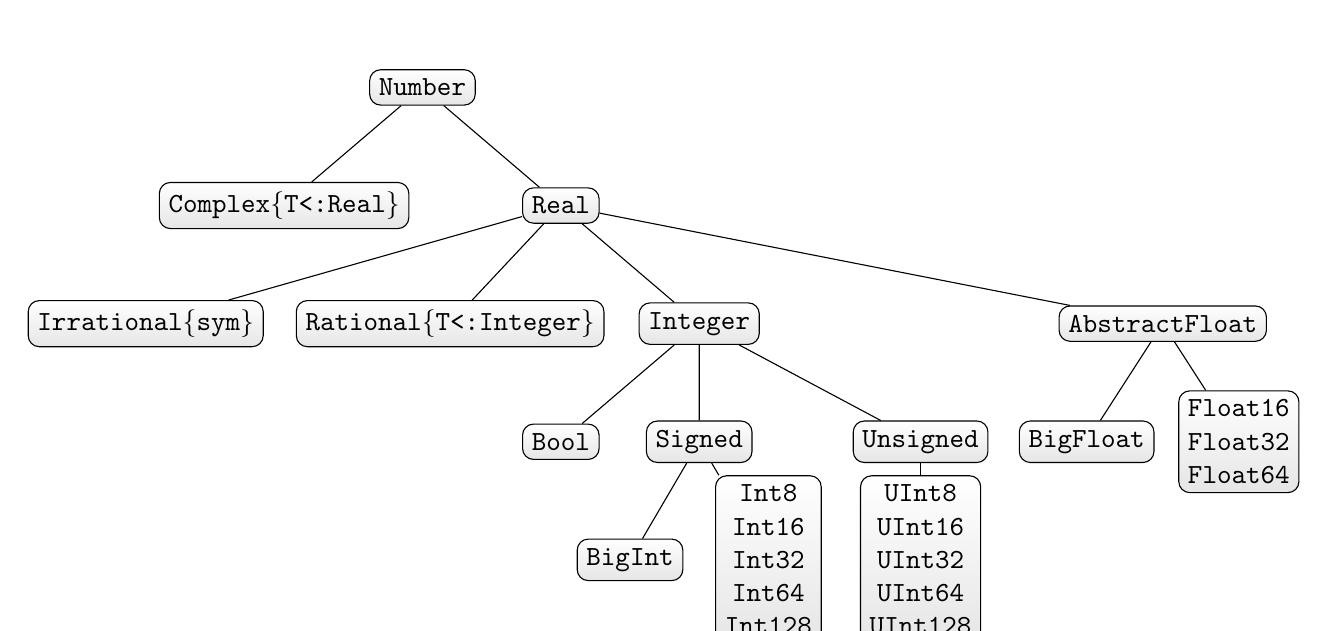
\begin{tikzpicture}[sibling distance=10em,
  every node/.style = {shape=rectangle, rounded corners,
    draw, align=center, font=\ttfamily,
    top color=white, bottom color=gray!20}]]
  \node {Number}
    child { node {Complex\{T<:Real\}} }
    child { node {Real}
        child { node {Irrational\{sym\}}}
        child[sibling distance=8em]{ node {Rational\{T<:Integer\}}}
        child { node {Integer}
            child[sibling distance=5em]{ node {Bool} }
            child[sibling distance=5em]{ node {Signed}
                child { node {BigInt} }
                child { node {Int8 \\ Int16 \\ Int32 \\ Int64 \\ Int128} }
            }
            child[sibling distance=8em]{ node {Unsigned}
                child[sibling distance=100em] { node {UInt8 \\ UInt16 \\ UInt32 \\ UInt64 \\ UInt128} }
            }
        }
        child[sibling distance=14.5em]{ node {AbstractFloat}
            child[sibling distance=5.5em]{ node {BigFloat} }
            child[sibling distance=5.5em]{ node {Float16 \\ Float32 \\ Float64} }
        }
    };
\end{tikzpicture}
\caption{数值类型的层级结构\label{fig:numeric}}
\end{figure}

全部标准数值类型的层级结构见图~\ref{fig:numeric}。

Julia 当然支持常见的数学运算和函数,我们可以把 Julia REPL 当作计算器使用。
\lstinputlisting{src/calc.jl}

Julia 遵循基本的算术运算优先顺序,以及一些省略乘号的语法糖,但依然推荐您在任何有必要的情况加括号。

\subsection{变量或名字}
上述常量都可以存到变量中,例如 \lstinline|x=3.4|。

在 Julia 中,变量应该被简单地理解为“名字”。
变量只是一笔数据的代号,本身并不和特定的类型有一对一的关系,
这和 Python 等动态语言一样,而和 C、FORTRAN 等语言不同。
因此,变量可以先后和不同类型的值绑定。
\lstinputlisting{src/variable.jl}


\section{更复杂的类型}
除基本类型以外,Julia 原生提供了多种实用的\textbf{复合类型}。
例如,上述复数即为复合类型。
除此之外,还有几种重要的复合类型。

\subsection{可索引的容器}
\textbf{元组}(Tuple)是不可变的序列,而\textbf{数组}(Array)是可变的序列。
而\textbf{可索引}是指可以用方括号来获得序列中的具体数值。
在 Julia 中,索引从 1 开始数,这和 FORTRAN、Matlab等一致,而和 C 不一样。
此外,元组和数组还有各种细微的区别,见下面的例子。
\lstinputlisting{src/tuple_array.jl}

根据作者的开发经验,元组(及\textbf{命名元组})更多用于函数与外部的交互。
故更多实例请见第\ref{sec:function}节。

\subsection{以数为内容的数组与线性代数}
以数为内容的数组可以理解为线性代数中的矢量和矩阵。
这部分是科学计算中的重点。
\lstinputlisting{src/linearalgebra.jl}

此外,Julia 支持\textbf{稀疏矩阵}和\textbf{分布式矩阵}。
分布式矩阵主要用于分布式计算中,本文不做介绍。
稀疏矩阵在科学计算中具有举足轻重的地位。
如果您的矩阵足够大又足够稀疏,且仅关心部分本征对,
应该考虑用稀疏矩阵。
\lstinputlisting{src/sparse.jl}

\subsection{字典}
字典(Dict)是一种关联容器[键(key)-- 值(value)对]:
\lstinputlisting{src/dict.jl}


\subsection{复合类型}
你可以定义、访问复合类型\textbf{复合类型}。以下是\textbf{可变}(mutable)复合类型的一个实例:
\lstinputlisting{src/struct.jl}

类似地,你可以通过删除 \lstinline|mutable| 关键字来定义\textbf{不可变}复合类型。 

你可以将你的类型定义为某抽象类型的子类型以将其适当的放在类型层级树中,
你也可以定义自己的抽象类型。



\subsection{字符串}
字符串(string)操作有:
\lstinputlisting{src/string.jl}

\lstinline|String| 和 \lstinline|SubString| 皆为 \lstinline|AbstractString| 的子类型。
\lstinline|SubString| 可避免复制字符串。
通常,当写自己的程序时,应假设用户会使用 \lstinline|AbstractString|。

注意!请避免索引字符串,例如 \lstinline|"Δ×a1=Ω"[3]|会是\lstinline|'×'| 而不是我们期待的\lstinline|'a'|。
这是因为Julia 是用 UTF-8 来编码标准字符串的,而索引是按字节而不是字符,
所以你需要理解UTF-8编码才能正确地索引。


\section{程序结构}

在逐行顺序执行所有语句外,可以用流程控制结构来控制执行的顺序。
常见的流程控制结构有 \lstinline|if|、\lstinline|while|、\lstinline|for| 等,
它们以块的形式出现。
在 Julia 中,块总是以 \lstinline|end| 结束,而有不同的开头。
\lstinputlisting{src/control.jl}

\section{函数}
\label{sec:function}

Julia 的\textbf{函数}(function)仅指抽象的接口,
具体的如 C 语言那样针对特定参数类型的具体执行过程则被称为\textbf{方法}(method)。
程序执行时,Julia 会根据你的参数类型调用特定的方法,这被称为\textbf{派发}(dispatch)。
Julia 中函数的定义是很灵活的,我们来看具体实例。
\lstinputlisting{src/function.jl}
从上面的例子可以看出 Julia 的函数调用的派发特性。
利用这个特性,我们可以方便地对不同类型的参数进行类似的操作。
如果一组类型的对象都遵循一样的运算逻辑,而其基础的运算规则都已经定义好,
不妨多多依赖 Julia 的派发机制。
Julia 的派发已经充分考虑了性能问题。
\lstinputlisting{src/dispatch_perform.jl}

\begin{lstlisting}
  f(x, y = 10) = x + y           # 新函数 f 的单行定义,y 默认值是 10
                                 # 返回最后一个表达式的结果
  function f(x, y=10)            # 和上面一样,但允许多个表达式
      x + y                      # 在函数体内
  end
  f(3, 2)                        # 简单的调用,返回 5
  f(3)                           # 返回 13
  (x -> x^2)(3)                  # 匿名函数的调用
  () -> 0                        # 没有参数的匿名函数
  h(x...) = sum(x)/length(x) - mean(x) # 可变参数的函数;x 是元组; 需要 using Statistics
  h(1, 2, 3)                     # 结果为 0
  x = (2, 3)                     # 元组
  f(x)                           # 错误:我们企图把10加到 (2, 3) 上
  f(x...)                        # 正确,元组解包
  s(x; a = 1, b = 1) = x * a / b # 有关键词参数 a 和 b 的函数
  s(3, b = 2)                    # 带关键词参数的调用
  q(f::Function, x) = 2 * f(x)   # 函数可以当作参数传递;这里我们要求 f 是一个函数
  q(x -> 2x, 10)                 # 返回 40,不必在 2x 中间写乘号(代表 2*x)
  q(10) do x                     # 通过 do 结构创建匿名函数,例如在输入输出有用
    2 * x
  end
  m = reshape(1:12, 3, 4)
  map(x -> x ^ 2, m)             # 包含转换过数据的 3x4 数组
  filter(x -> bitstring(x)[end] == '0', 1:12)  # 在区间里筛选偶数的亮眼方法
  ==(1)                          # 返回一个检查是否等于1的函数
  findall(==(1), 1:10)           # 找到所有等于 1 的元素的索引,相似地:findfirst, findlast
\end{lstlisting}

习惯上以 \lstinline|!| 结尾地函数会原位修改其参数。参见本文档中的 \lstinline|resize!|。

默认函数参数自左向右求值:
\begin{lstlisting}
  y = 10
  f1(x=y) = x; f1()      # 10
  f2(x=y,y=1) = x; f2()  # 10
  f3(y=1,x=y) = x; f3()  # 1
  f4(;x=y) = x; f4()     # 10
  f5(;x=y,y=1) = x; f5() # 10
  f6(;y=1,x=y) = x; f6() # 1
\end{lstlisting}

Julia 中\textsf{函数}可以有多个\textsf{方法}(method)。
每个方法对应函数的一组参数类型。
这种行为叫多重派发(multiple dispatch)并且只对位置(positional)参数有效。
以下是一些简短的例子。详见 Julia 的 Methods 章节。
\begin{lstlisting}
  g(x, y) = println("all accepted") # g 函数接收任何类型 x 和 y 的方法
  function g(x::Int, y::Int)        # 当 x 和 y 均为 Int 型调用的方法
    y, x
  end
  g(x::Int, y::Bool) = x * y        # 当 x 为 Int,y 为 Bool 时的方法
  g(1.0, 1)                         # 第一个定义被调用
  g(1, 1)                           # 第二个定义被调用
  g(1, true)                        # 第三个定义被调用
  methods(g)                        # 列出 g 的所有方法
  t(; x::Int64 = 2) = x             # 单个关键词参数
  t()                               # 返回 2
  t(; x::Bool = true) = x           # 没有对关键词参数的多重派发,函数定义被覆盖
  t()                               # true;旧函数被覆盖
\end{lstlisting}

\section{变量作用域}
以下结构创建新的变量作用域(variable scope):
\lstinline|function|、\lstinline|while|、
\lstinline|for|、\lstinline|try/catch|、
\lstinline|let|、\lstinline|struct|、\lstinline|mutable struct|。

你可以将变量定义为:
\begin{itemize}
  \item \lstinline|global|:在当前模块的全局作用域使用变量;
  \item \lstinline|local|: 在当前作用域定义新变量;
  \item \lstinline|const|: 确保变量类型是常量(仅全局)。
\end{itemize}

特殊情况:
\begin{lstlisting}
  t                  # 错误,变量 t 不存在
  f() = global t = 1
  f()                # 调用后 t 在全局作用域被定义

  function f1(n)
    x = 0
    for i = 1:n
      x = i
    end
    x
  end
  f1(10)            # 10;在循环内我们使用了外部局域变量

  function f2(n)
    x = 0
    for i = 1:n
      local x
      x = i
    end
    x
  end
  f2(10)            # 0;在循环内我们使用了新的局域变量

  function f3(n)
    for i = 1:n
      h = i
    end
    h
  end
  f3(10)            # 错误;h 在外部作用域未定义

  const x = 2
  x = 3 # 警告,常量的值被改变;但你永远不应该这样写,这会导致编译好的代码失效
  x = 3.0 # 错误,类型错误

  function f()
      x::Int = 1
      x = 2.5 # 当调用 f() 时会报错,因为 x 必须是 Int
  end
\end{lstlisting}
全局常量会加速代码执行,因为编译器知道其类型。

循环和推导在每次迭代时都重新给变量赋值,故可以安全地在迭代中用他们创造闭包(closure):
\begin{lstlisting}
  Fs = Array{Any}(undef, 2)
  for i in 1:2
    Fs[i] = () -> i
  end
  Fs[1](), Fs[2]() # (1, 2)
\end{lstlisting}

\section{模块}
模块(module)将代码封装起来,每个模块有他们自己的全局命名空间(Julia REPL 的模块名是 \lstinline|Main|)。
\begin{lstlisting}
  module M # 模块名
  export x # 模块向外界所暴露的
  x = 1
  y = 2 # 隐藏变量
  end

  varinfo(M) # 列出导出的变量
  x       # 在全局作用域中找不到
  M.y     # 可以直接访问变量

  # 导入所有导出的变量
  # 也可以用此法加载标准包,但不需要 . 前缀
  using .M

  # 将 y 导入全局作用域 (即使其没有被导出)
  import .M.y
\end{lstlisting}
给其他模块中的变量绑定值是不可以的。如下是常常让人们惊讶的经典小例子:
\begin{lstlisting}
  sin(1) # 成功
  sin = 1 # 失败,在模块 Main 里你不能给模块 Base 里的变量绑定值
  cos = 1 # 成功,因为cos还没有被调用,故还没有从 Base 导入到 Main
  cos # 返回 1
  cos(1) # 失败,cos 在 Main 模块绑定了 1
  Base.cos(1) # 成功
\end{lstlisting}

\section{操作符}
Julia 使用标准的操作符,而有如下的小技巧:
\begin{lstlisting}
  true || false    # 二元或算符(仅单元素使用),|| 和 && 采短路求值
  [1 2] .& [2 1]   # 逐位(bitwise)与算符 [以 . 向量化(vectorize)]
  1 < 2 < 3        # 支持连锁条件(chaining conditions)(仅单元素使用,不可用 . 向量化)
  [1 2] .< [2 1]   # 向量化的操作符需要前缀 .
  x = [1 2 3]
  2x + 2(x .+ 1)   # 字面值和变量间的乘号及字面值或变量与左括号间的乘号可省略
  y = [1, 2, 3]
  x + y  # 错误:维度不匹配
  x .+ y # 3x3 矩阵,维度广播(broadcasting)
  x + y' # 1x3 矩阵
  x * y  # 数组乘法,单元素矢量(不是标量)
  x .* y # 逐元素(element-wise)乘法,3x3 数组

  x == [1 2 3]  # true,对象值一样
  x === [1 2 3] # false,对象并非同一

  z = reshape(1:9, 3, 3)
  z + x  # 错误:维度不匹配
  z .+ x # x 纵向广播
  z .+ y # y 横向广播

  # 长度为1的维度的显式广播
  # 对每一个数组元素,函数 + 都被调用
  broadcast(+, [1 2], [1; 2])
  # 使用 . 操作符广播
  using Random
  length([randstring(10) for i in 1:5]) # 5:数组的长度
  length.([randstring(10) for i in 1:5]) # 由 10 构成的 5个元素的数组:字符串的长度
\end{lstlisting}

函数广播的例子:
\begin{lstlisting}
  t(x::Float64, y::Float64 = 1.0) = x * y
  t(1.0, 2.0)               # 成功
  t([1.0 2.0])              # 错误
  t.([1.0 2.0])             # 成功
  t([1.0 2.0], 2.0)         # 错误
  t.([1.0 2.0], 2.0)        # 成功
  t.(2.0, [1.0 2.0])        # 成功
  t.([1.0 2.0], [1.0 2.0])  # 成功
  t.([1.0, 2.0], [1.0 2.0]) # 成功
\end{lstlisting}

\section{基本常用函数}
\begin{lstlisting}
  show(collect(1:100)) # 显示对象的字符串表示
  eps()             # 从 1.0 到下一个可表示的 Float64 类型数的差距(译注:机器相对误差)
  nextfloat(2.0)    # 下一个可表示的浮点数,类似地,提供了 prevfloat
  isequal(NaN, NaN) # true
  NaN == NaN        # false
  NaN === NaN       # true
  isequal(1, 1.0)   # true
  1 == 1.0          # true
  1 === 1.0         # false
  0.0 == -0.0       # true
  0.0 === -0.0      # false
  isfinite(Inf)     # false,类似地提供了 isinf, isnan
  fld(-5, 3), mod(-5, 3) # (-2, 1), 朝向负无穷的整数除法
  div(-5, 3), rem(-5, 3) # (-1, -2), 朝向零的整数除法
  findall(x -> mod(x, 2) == 0, 1:8) # 找到使函数为真的索引
  x = [1 2]; identity(x) === x # true,返回参数本身
  @info "Info"      # 打印信息,类似地有 @warn 和 @error (参见 Logging 模块)
  ntuple(x->2x, 3)  # 通过以值 1、2、3 调用 x->2x 创建元组
  @isdefined x      # 变量 x 是否被定义
  y = Array{Any}(undef,2); isassigned(y, 3)  # 数组中的第3位是否被赋值(而不是越界或者 #undef)
  fieldtype(typeof(1:2),:start) # 获取复合类型中域的类型(以符号传参)
  fieldnames(typeof(1:2)) # 获取类型中域的名称
  zip(1:3, 1:3) |> collect # 将迭代器打包为迭代器元组,并且将其传给 collect 函数
  enumerate("abc")  # 创建能够遍历由索引和内容元素构成的元组的迭代器
  collect(enumerate("abc")) # 并将其转换为数组
  isempty("abc")    # 检查一个组合是否为空;字符串视为字符的组合
  'b' in "abc"      # 检查元素是否在组合里
  indexin(collect("abc"), collect("abrakadabra")) # [1, 2, nothing] ('c' 没有找到),需要数组
  findall(in("abrakadabra"), "abc") # [1, 2] ('c' 没有找到)
  unique("abrakadabra") # 舍去重复的元素
  issubset("abc", "abcd") # 检查是否第一个组合里的每一个元素都在第二个组合里(译注:判断是否为子集)
  argmax("abrakadabra") # 最大元素的索引(3:对应'r')
  findmax("abrakadabra") # 最大元素及其索引构成的元组
  filter(x->mod(x,2)==0, 1:10) # 保留一个组合里满足条件的元素
  dump(1:2:5)       # 显示该对象所有对用户可见的结构
  sort(rand(10))    # 对 10 个随机数排序,sort! 可进行原位排序
\end{lstlisting}

\section{读写数据}
有关输入输出的细节,见 Julia 文档。有大量的包提供了该功能。
\lstinline|DelimitedFiles| 模块中的基本操作有:
\begin{itemize}
  \item \lstinline|readdlm|:从文件读
  \item \lstinline|writedlm|:写入文件
\end{itemize}

警告!如果文件读取时设置\lstinline|delim=' '|,则空格不会被忽略。

\section{随机数}
基本的随机数用法:
\begin{lstlisting}
  Random.seed!(1) # 设定随机数种子为 1;需要先调用 using Random
  rand()        # 在 U[0,1) 范围内生成随机数
  rand(3, 4)    # 在 U[0,1) 范围内生成 3x4 随机数矩阵
  rand(2:5, 10) # 在 2 到 5 范围内生成 10 个随机整数构成的数组
  randn(10)     # 依正态分布生成 10 个随机数构成的数组
\end{lstlisting}

\lstinline|Distributions| 包中的进阶随机数:
\begin{lstlisting}
  using Distributions # 加载包
  sample(1:10, 10)    # 从集合 1 到 10 中的随机取样
  b = Beta(0.4, 0.8)  # 参数为 0.4 和 0.8 的 beta 分布
                      # 支持的分布详见文档
  mean(b)             # b 分布的期望值
                      # 支持的统计详见文档
  rand(b, 100)        # b 分布下100个独立随机取样
\end{lstlisting}

\section{统计与机器学习}
访问 \url{http://juliastats.github.io/} 获取更多信息(尤其是类似于 R 语言的数据框架)。

Julia 中的一个核心语言结构 \lstinline|Missing| 专门用于表示缺失的值。
\begin{lstlisting}
  missing # 缺失的值
  ismissing(missing) # true
  coalesce(missing, 1, 2) # 返回第一个没有缺失的值,当所有值都缺失的时候返回 missing
\end{lstlisting}

\section{宏}
你可以定义宏(macro)(详见文档)。有用的标准宏有:

断言:
\begin{lstlisting}
  @assert 1 == 2 "ERROR"            # 2 个宏参数,引发错误
  using Test                        # 加载 Test 包
  @test 1 == 2                      # 与 assert 类似;错误similar to assert; error
  @test_throws DomainError sqrt(-1) # 通过,不可以使用 sqrt(-1)
\end{lstlisting}

基准测试:
\begin{lstlisting}
  @time [x for x in 1:10^6];    # 打印出所用时间和内存
  @timed [x for x in 1:10^6];   # 返回值、时间和内存
  @elapsed [x for x in 1:10^6]   # 返回时间
  @allocated [x for x in 1:10^6] # 返回内存
\end{lstlisting}
使用 \lstinline|BenchmarkTools| 包以获得更强大的基准测试功能。

\section{绘图}
\label{sec:plot}
Julia 有几个绘图包,例如 \lstinline|Plots| (涵盖了多个绘图后端的接口包)以及 \lstinline|PyPlot|.
这里我们介绍 Python 用户会觉得似曾相识的 \lstinline|PyPlot|。
\begin{lstlisting}
  using PyPlot
  using Random
  Random.seed!(1) # 使绘图可重现
  x, y = randn(100), randn(100)
  scatter(x, y)
\end{lstlisting}

我们从\url{https://matplotlib.org/1.2.1/examples/pylab_examples/histogram_demo.html}借用一个例子:
\begin{lstlisting}
  using Distributions
  using PyPlot

  mu, sigma = 100, 15
  x = mu .+ sigma * randn(10000)

  n, bins, patches = plt.hist(x, 50, density=1,
      facecolor="green", alpha=0.75)

  y = pdf.(Ref(Normal(mu, sigma)), bins);
  plot(bins, y, "r--", linewidth=1)

  xlabel("Smarts")
  ylabel("Probability")
  title(raw"$\mathrm{Histogram\ of\ IQ:}\ \mu=100,\ \sigma=15$")
  axis([40, 160, 0, 0.03])
  grid(true)
\end{lstlisting}

产生:


\section{处理表格数据}

Julia 里有多个包支持表格数据。

这里我们介绍 \lstinline|DataFrames| (0.21 版) 和 \lstinline|CSV| 两个包。

加载一个逗号分隔表(CSV)文件:
\begin{lstlisting}
  using DataFrames
  using CSV
  path = joinpath(dirname(pathof(DataFrames)), "../docs/src/assets/iris.csv")
  df = DataFrame(CSV.File(path));
  first(df, 5) # 打印数据中的前5行;使用 last 函数来打最后几行
\end{lstlisting}

生成如下的输出:
\begin{lstlisting}
  4x5 DataFrame
  | Row | SepalLength | SepalWidth | PetalLength | PetalWidth | Species     |
  |     | Float64     | Float64    | Float64     | Float64    | String      |
  |-----+-------------+------------+-------------+------------+-------------|
  | 1   | 5.1         | 3.5        | 1.4         | 0.2        | Iris-setosa |
  | 2   | 4.9         | 3.0        | 1.4         | 0.2        | Iris-setosa |
  | 3   | 4.7         | 3.2        | 1.3         | 0.2        | Iris-setosa |
  | 4   | 4.6         | 3.1        | 1.5         | 0.2        | Iris-setosa |
\end{lstlisting}

读入\lstinline|DataFrame| 后,让我们介绍几条处理它的最有用的几个操作:
\begin{lstlisting}
  DataFrame(a=1:10, b=rand(10)) # 由几组数据手动生成 DataFrame
  describe(df) # 获取数据框架的概要信息
  df.Species # 获取 df 中的 Species 字段而不进行复制操作
  df[!, :Species] # 同上
  df[1, 5] # 从数据框架中获取第1行第5列的值
  df[1:2, 1:2] # 创建数据框架的子集,由前两行的前两列构成
  Matrix(df[:, 1:4]) # 将第1到第4列转换为矩阵
  names(df) # 以字符串形式获取数据框架中的字段名
  nrow(df), ncol(df) # 数据框架的行数和列数number of rows and columns in a data frame
  sort(df, :SepalWidth) # 返回一个以 SepalWidth 排序的新数据框架
  filter(:SepalWidth => >(3), df) # 返回一个仅包含满足预设条件的行的新数据框架
  push!(df, (1, 2, 3, 4, "Some species")) # 在数据框架的末尾加一新行
  df.key = axes(df, 1) # 向数据框架中添加一个新变量 key

  # 按 Species 计算 SepalLength 的总和,并将结果存在 x 中
  combine(groupby(df, :Species), :SepalLength => sum)

  # 把 df 转变成以 SepalLength 为值而 key 与 Species 对为 id 的长格式
  df2 = stack(df, :SepalLength, [:key, :Species])
  unstack(df2) # 相反的操作:宽到长格式
\end{lstlisting}


\section{扩展阅读}
\label{sec:readmore}

请参阅 Julia 最新版文档 \url{https://docs.julialang.org/} 
\footnote{译注:亦可参考完善中的中文文档 \url{https://docs.juliacn.com/latest/},但请以英文原文为准。} 以了解这些内容。

\end{document}
